\documentclass[11pt]{beamer}
\usetheme{Warsaw}
\usepackage[utf8]{inputenc}
\usepackage[english]{babel}
\usepackage{amsmath}
\usepackage{amsfonts}
\usepackage{amssymb}
\usepackage[]{algorithm2e}
\usepackage{animate}
\usepackage{scrextend}
\usepackage{booktabs}
\usepackage{hyperref}
\usepackage{graphicx}
\usepackage{subcaption}
\usepackage{tcolorbox}
\usepackage{lipsum}
\usepackage{systeme}
\usepackage{multirow}


\author{Chan Hei Nam, \\Cheng Tin Chu, \\Lei Wen Feng, \\Ng Wing Hin}

\title{Ranking and Prediction of Amazon Fine Food based on Costumer's rating and review}
\date{}
%\setbeamercovered{transparent}
%\setbeamertemplate{navigation symbols}{}
%\logo{}
%\institute{}
%\date{}
%\subject{}
\begin{document}

\theoremstyle{plain}
\newtheorem{thm}{Theorem}[section] % reset theorem numbering for each chapter

\theoremstyle{definition}
\newtheorem{defn}[thm]{Definition} % definition numbers are dependent on theorem numbers
\newtheorem{exmp}[thm]{Example} % same for example numbers
\newtheorem{prop}{Property}[section]

\graphicspath{ {images/} }

\begin{frame}
\titlepage
\end{frame}

%\begin{frame}
%\tableofcontents
%\end{frame}

\begin{frame}
\frametitle{Introduction}
User's rating and review is one of the explicit ways to determine product's popularity. In this project, we are trying to process the Amazon Fine Food Reviews such that the result can be used to predict the rating based on review.
\end{frame}

\begin{frame}
\frametitle{Basic statistics of the dataset}

\begin{tcolorbox}[colback=blue!5,colframe=blue!40!black,title=Basic statistics of the dataset]
\centering
\begin{tabular}{lll}
	\hline
	    					& Rating 	& Word(Processed)\\
	\hline
	Mean					& 4.18 		& 255\\
%	Standard Deivation	& 1.31		& \\
	Minimum       		& 1 			& 7\\
	Maximum       		& 5 			& 14425\\
%	First Quartile 		& 4 			& 				& \\
%	Median 				& 4 			& 				& \\
%	Third Quartile 		& 5 			& 				& \\
	\hline
\end{tabular}
\end{tcolorbox}
\end{frame}


\begin{frame}
\frametitle{System Structure}
There are mainly three stages in our system :
\begin{labeling}{alligator}
\item [Stage 1] Pre-processing the dataset.
\item [Stage 2] Using MapReduce, find the first hundred k-shingles, \(1\leq k\leq 5\), of each rating, \(1 \leq \mbox{rating} \leq 5\).
\item [Stage 3] Do prediction of rating based on the review input to the system.
\end{labeling}
\end{frame}


\begin{frame}
\frametitle{Stage 1 Pre-processing}

\begin{tcolorbox}[colback=blue!5,colframe=blue!40!black,title=\textbf{Algorithm 1}: Pre-processing]
\begin{algorithm}[H]
 \While{There exists next row inside Reviews.csv}
 {
 	Extract \textbf{Rating} and \textbf{Text}\;
 	Lower \textbf{Text} and remove \emph{some} stopwords and punctuation\;
 	Returning line with format \(Rating, word_{1}, word_{2}, ...\)\;
 }
\end{algorithm}
\end{tcolorbox}

\end{frame}

\begin{frame}
\frametitle{Example result from Stage 1}

Original data :

\vspace{2mm}

\resizebox{\linewidth}{!}{
\begin{tabular}{l}
  \toprule
	Id, ProductId, UserId, ProfileName, HelpfullnessNumerator, HelpfullnessDenominator, Score, Time, Summary, Text\\
  \midrule
	1,B001E4KFG0,A3SGXH7AUHU8GW,delmartian,1,1,5,1303862400,Good Quality Dog Food,I have bought... \\
	2,B00813GRG4,A1D87F6ZCVE5NK,dll pa,0,0,1,1346976000,Not as Advertised,"Product arrived labeled...\\
	3,B000LQOCH0,ABXLMWJIXXAIN,"Natalia Corres ""Natalia Corres""",1,1,4,1219017600,"""Delight"" says it all","This is a confection...\\
    4,B000UA0QIQ,A395BORC6FGVXV,Karl,3,3,2,1307923200,Cough Medicine,If you are looking... \\

  \bottomrule

\end{tabular}}

\vspace{5mm}


Result data :

\vspace{2mm}

\resizebox{\linewidth}{!}{
\begin{tabular}{l}
  \toprule
	Score, Text\\
  \midrule
 	5,bought vitality canned dog food products good quality product looks... \\
	1,product arrived labeled jumbo salted peanutsthe peanuts actually... \\
	4,confection centuriesit light pillowy citrus gelatin nutsin case filberts...\\
	2,looking secret ingredient robitussin believe iti got addition root... \\
  \bottomrule
\end{tabular}}
\end{frame}

\begin{frame}
\frametitle{Stage 2 MapReduce}

\begin{tcolorbox}[
	colback=blue!5,
	colframe=blue!40!black,
	title=\textbf{Algorithm 2}: MapReduce (Mapper)
	]
\begin{algorithm}[H]
	\While{There exists next row inside Preprocessed.csv}
	{
		\For{$k \leftarrow 1$ \KwTo $5$}
		{
			\label{forins}
			Find all k-shingles\;
			\For{Each shingle found}
			{
				Return \(<<\mbox{rating, k, shingle}>, 1>\);
			}
 		}
	}
\end{algorithm}
\end{tcolorbox}

\end{frame}

\begin{frame}
\frametitle{Stage 2 MapReduce}

\begin{tcolorbox}[
	colback=blue!5,
	colframe=blue!30!black,
	title=\textbf{Algorithm 2}: MapReduce (Reducer)
	]
\begin{algorithm}[H]
	\ForAll{tuples with key \(<\mbox{rating, k, shingle}> \)} {
		frequency = sum of all tuple values\;
		Return \(<\mbox{rating, k, frequency, shingle}>\)\;
	}
\end{algorithm}
\end{tcolorbox}

\end{frame}

\begin{frame}
\frametitle{Exmaple result from Stage 2}

Result from MapReduce : \\
\vspace{5mm}
\resizebox{\linewidth}{!}{
\begin{tabular}{llll}
  \toprule
	Score& k& frequency& shingle\\
  \midrule
	3&4&23&food freshly openedpi likes\\
	1&2&238&br tried\\
	2&1&1601&say\\
	3&4&27&coffeetea love organic coffee\\

  \bottomrule

\end{tabular}}

\end{frame}


\begin{frame}
\frametitle{Stage 3 Prediction}

	\begin{tcolorbox}[
		colback=blue!5,
		colframe=blue!40!black,
		title=\textbf{Algorithm 3}: Prediction using length-k shingles]

		\begin{algorithm}[H]

			Load the \(records\) from \textbf{Shingle Database}\;
			Find all \textit{k-shingles} in the input text\;
			\ForEach{shingle}
			{
				Collect all records of \textit{shingle} from database\;
				Append to \(RecordsFound\)\;
			}
			\eIf {\(RecordsFound\) is not empty}
			{
				\(score\) = weighted average of \(RecordsFound\)\;
			}
			{
				\(score\) = average of all records in database\;
			}
			return \(score\)\;

		\end{algorithm}

	\end{tcolorbox}

\end{frame}


\begin{frame}
\frametitle{Stage 3 Prediction}

	\begin{tcolorbox}[
		colback=blue!5,
		colframe=blue!40!black!60,
		title=Prediction Example]

		Database:
		\begin{center}
			\begin{tabular}{llll}
			  \toprule
					Score & k & frequency & shingle \\
			  \midrule
					5 & 1 & 68 & good \\
					4 & 1 & 35 & good \\
					5 & 1 & 57 & really \\
			  \bottomrule
			\end{tabular}
		\end{center}

		Input: \textit{this is \underline{really} \underline{good}} \\
		Score:
		\begin{center}
			\(\frac{5 \times 68 + 4 \times 35 + 5 \times 57}{68 + 35 + 57}\) = 4.78125
		\end{center}

	\end{tcolorbox}
\end{frame}

\begin{frame}
\frametitle{Demostration}

	\begin{center}
		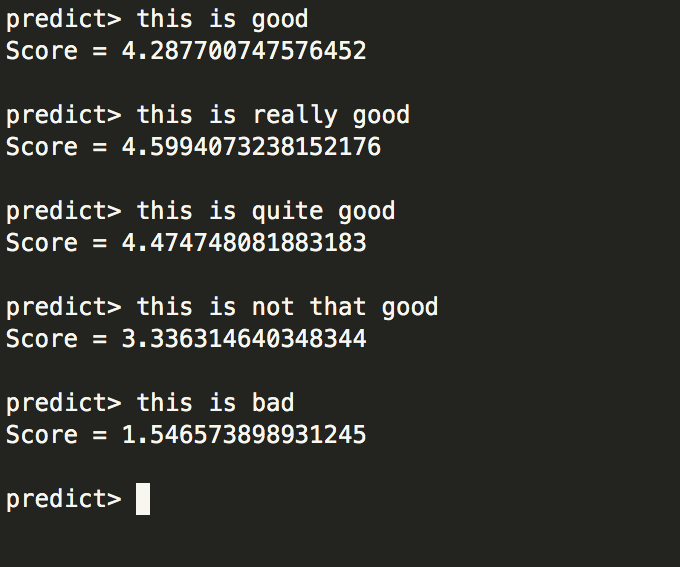
\includegraphics[width=7.5cm]{demo} \\
		Video Demo: \url{https://goo.gl/fqaTSo}
	\end{center}

\end{frame}


\begin{frame}
\frametitle{Stage 3 Prediction}

	Using shingles of different lengths, we got different performances:

	\begin{center}
		\begin{tabular}{cc}
			\toprule
				Shingle Length & Mean Squared Error \\
			\midrule
				1 & 1.596 \\
				2 & 2.160 \\
				3 & 2.918 \\
				4 & 3.089 \\
				5 & 3.112 \\
			\bottomrule
		\end{tabular}
	\end{center}
	\vspace{5mm}
	But we need to respect shingles of different length. How?

\end{frame}

\begin{frame}
\frametitle{Regression Model}
\begin{tcolorbox}[colback=blue!5,colframe=blue!40!black,title=Regression model]
Regression equation :
\begin{equation}
\begin{alignedat}{1}
y &= \beta_0  + \beta_1 x_1 + \dots + \beta_5 x_5\\
\end{alignedat}
\end{equation}
where $x_i$ is the $i$-th shingle score, for $i=1,...,5$
\end{tcolorbox}
\end{frame}



\begin{frame}
\frametitle{Regression Model}
\begin{tcolorbox}[colback=blue!5,colframe=blue!40!black,title=Regression model]
System of linear equation :
\begin{equation}
\begin{alignedat}{4}
y_1 &= \beta_0  + \beta_1 x_{11} + \dots + \beta_5 x_{15}\\
y_2 &= \beta_0 + \beta_1 x_{21} + \dots + \beta_5 x_{25}\\
\;\vdots  &            \qquad\qquad\qquad\vdots \\
y_n &= \beta_0 + \beta_1 x_{n1} + \dots + \beta_5 x_{n5}
\end{alignedat}
\end{equation}
In matrix form :

\centering
\(\textbf{Y}= \boldsymbol{\beta_0}+\textbf{X} \cdot \boldsymbol{\beta} \)

\raggedright
where\\
\(\textbf{Y}\) is a \(n\times1\) matrix,\\
\(\boldsymbol{\beta_0}\) is a \(n\times 1\) matrix,\\
\(\boldsymbol{\beta}\) is a \(5\times 1\) matrix,\\
\(\textbf{X}\) is a \(n\times 5\) matrix.
\end{tcolorbox}
\end{frame}



\begin{frame}
\frametitle{Regression Model}
\begin{tcolorbox}[colback=blue!5,colframe=blue!40!black,title=Complexity]
key computation step:
\begin{itemize}
\item \(\textbf{X}^T\textbf{X} \mbox{ in O(} n\times k^2 \mbox{)}\)
\item \((\textbf{X}^T\textbf{X})^{-1} \mbox{ in O(} k^3 \mbox{)}\)
\end{itemize}
n = number of rows from train data\\
k = number of regression parameters = 5\\
As \(n>>k\), the overall complexity is O(\(n\)).
\end{tcolorbox}
\end{frame}



\begin{frame}
\frametitle{Result}

	\centering
	Shingle Match Performance

	\begin{center}
		%\begin{tabular}{11}
		\begin{tabular}{cc}
			\toprule
				Shingle Length & Match \% \\
			\midrule
				1 & 99.87\% \\
				2 & 67.88\% \\
				3 & 16.47\% \\
				4 & 2.19\% \\
				5 & 0.30\% \\
			\bottomrule
		\end{tabular}
	\end{center}
	\vspace{5mm}




\end{frame}

\begin{frame}
\frametitle{Result(Cont'd)}

	\centering
	Performance - MSE comparison

	\begin{center}
	
		\begin{tabular}{ccc}
			\toprule
				\multirow{2}{*}{Prediction Method} &
				\multicolumn{2}{c}{Default Score}\\
				\cline{2-3}
				& 3 & Train Mean = 4.18 \\
				%Method & testing \\
			\midrule
				Train Data Mean & 1.717 & 1.717 \\
				\hline
				1-shingle & 1.596 & 1.596\\
				2-shingle & 2.160 & 1.595\\
				3-shingle & 2.918 & 1.667\\
				4-shingle & 3.089 & 1.704\\
				5-shingle & 3.112 & 1.710\\
				\hline
				Regression & 1.449 & 1.369\\
				
			\bottomrule
		\end{tabular}
	\end{center}
	\vspace{5mm}

\end{frame}

\begin{frame}
\frametitle{Result(Cont'd)}

\begin{figure}[h!]
  \centering
  Error Spread of 1-shingle\\
  \begin{subfigure}[b]{0.45\textwidth}
    \caption{Default Score = 3}
    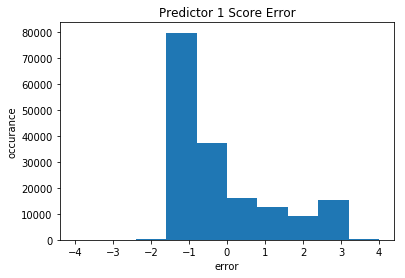
\includegraphics[width=\linewidth]{predictor_1_error_3}
  \end{subfigure}
  \begin{subfigure}[b]{0.45\textwidth}
    \caption{Default Score = 4.18}
    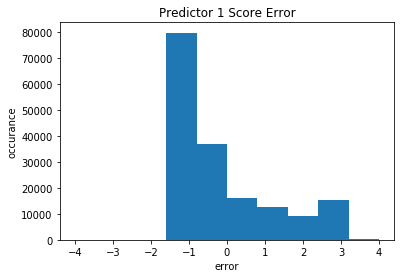
\includegraphics[width=\linewidth]{predictor_1_error_train_mean}
  \end{subfigure}
\end{figure}

\end{frame}

\begin{frame}
\frametitle{Result(Cont'd)}

\begin{figure}[h!]
  \centering
  Error Spread of 5-shingle\\
  \begin{subfigure}[b]{0.45\textwidth}
    \caption{Default Score = 3}
    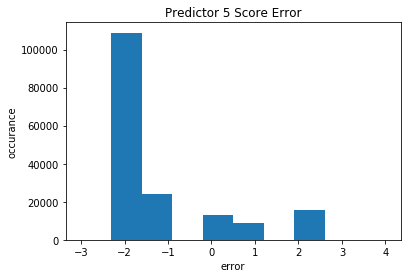
\includegraphics[width=\linewidth]{predictor_5_error_3}
  \end{subfigure}
  \begin{subfigure}[b]{0.45\textwidth}
    \caption{Default Score = 4.18}
    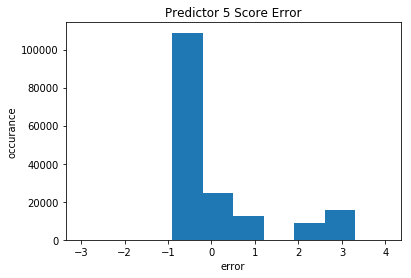
\includegraphics[width=\linewidth]{predictor_5_error_train_mean}
  \end{subfigure}
\end{figure}

\end{frame}

\begin{frame}
\frametitle{Result(Cont'd)}

\begin{figure}[h!]
  \centering
  Error Spread of Regression Method\\
  \begin{subfigure}[b]{0.45\textwidth}
    \caption{Default Score = 3}
    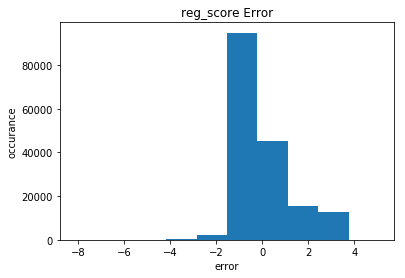
\includegraphics[width=\linewidth]{reg_error_3}
  \end{subfigure}
  \begin{subfigure}[b]{0.45\textwidth}
    \caption{Default Score = 4.18}
    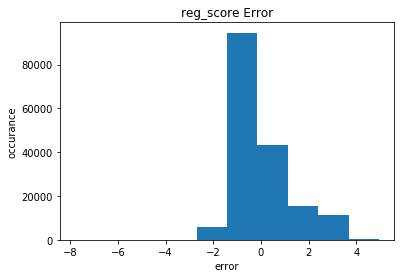
\includegraphics[width=\linewidth]{reg_error_train_mean}
  \end{subfigure}
\end{figure}

\end{frame}


\begin{frame}
\frametitle{Conclusion}
	
	\begin{itemize}
		\setbeamertemplate{itemize items}[square]
		\item Use Train Data Mean as default score.
		\item The higher the match \%, the more accurate prediction.
		\item 1-shingle method is better than other k-shingle methods.
		\item Regression method is the best method.
	\end{itemize}		
	

	


\end{frame}

\end{document}
